

\input{paramètres}

\begin{document}


\begin{center}
\vspace*{2cm}

{\TitleFont\LARGE Fiche}\\[1em]
{\TitleFont\Huge DCF MODEL VALUATION}\\[1em]
{\TitleFont\large ESCP Business School}\\[2em]

\textsc{---}\\[1em]
\textsc{Étudier pour Comprendre, Comprendre pour Servir}\\[2em]

{\SmallCapsFont Fiche de cour}\\[0.5em]
{\small A partir du cours d'Aswath Damodaran}\\[2em]

{\SmallCapsFont Par}\\[0.5em]
{\Large V. VITRAC}\\
{\footnotesize Etudiant ESCP et ancien Fermatien}\\[2em]

{\normalsize Thème : Finance}\\[2em]

{\Large\textbf{PROGRAMME ACTUEL}}\\[2em]

% Logo EB dessiné rapidement avec TikZ pour simuler
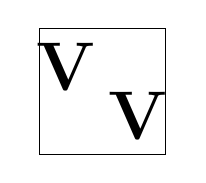
\begin{tikzpicture}
\node at (0,0) {\Huge$^\textbf{V} \,_\textbf{V}$};
\draw (-0.8,0.8) rectangle (0.8,-0.8);
\end{tikzpicture}\\[2em]

{\Large PARIS}\\[0.5em]
{\small Années 2025-2026} 

\vspace{5mm}

{\scriptsize Droits de traduction et de reproduction réservés}
\end{center}





\newpage
\onehalfspacing


% Declare paragraph level for ToC
\newlength{\cftparagraphindent}
\setlength{\cftparagraphindent}{110pt} % No indent
\newlength{\cftparagraphnumwidth}
\setlength{\cftparagraphnumwidth}{4.6em} % Adjust number width if needed

\cftsetindents{paragraph}{\cftparagraphindent}{\cftparagraphnumwidth}


\tableofcontents

\newpage


%---------------------------------
% Chapitre 1


\chapter*{Forewords}




\begin{center}
    \textit{The DCF is like a Hubble telescope — if you turn one knob a little,\\ you end up in a different galaxy} 

    ---------\\
    \textbf{Aswath Damodaran}
\end{center}

\vfill

\lettrine{A}{} valuation method always aims to determine the value of an asset or a company. However, all valuations are biased: the exact price will never be found. The only question is how far you are from the truth—and how your bias depends on who is paying you. Hence, all valuations are only meant to provide an estimated value. Such a model doesn't need a vast number of inputs to be useful: keeping things understandable is the key to an effective valuation. The DCF (Discounted Cash Flow) model aims to estimate the value of an asset or business based on the present value of its expected future cash flows. Therefore, assets or businesses with strong near-term cash flows will be valued more highly than those with later cash flows. When valuing a company, the analyst aims to determine the total value of the business—not just the equity, but also the claims held by other stakeholders. The DCF model operates under the assumption of market inefficiency: prices are not perfect and do not reflect all available information. The market is therefore expected to make pricing mistakes and to correct them over time as new information emerges.




\chapter{Presentation of the model}

The core of the model relies on the discounting of future cash flows. Throughout this document, we will use $t$ as a marker of time and $CF_t$ to denote the cash flow at time $t$. The principle of the model is to discount the business’s cash flows based on growth assumptions and a discount rate. Therefore, the first statement is that for a business to have a positive value, it must generate positive cash flows. The cash flows we use are free cash flows (which we could denote as $FCFF_t$, but for simplicity, we will use $CF_t$).

\section{The inputs of the model}

Depending on whether we are valuing an asset or a firm, the required inputs differ slightly. To value equity, we use the cost of equity; to value a firm, we use the cost of capital. Additionally, depending on whether the cash flows are expressed in nominal or real terms, we must use a corresponding nominal or real discount rate. Once the discount rate is established (noting that it may vary over time), we must compute both current and projected earnings and cash flows, which involves making assumptions about risk and growth. Ultimately, we also need to estimate when the company’s growth will stabilize, and under which risk and cash flow parameters this will occur.

\subsection{The discount rate}

The discount rate is a key variable in the DCF model. A small change in its estimation can lead to significant variation in the final valuation result. The cornerstone of an accurate discount rate estimation is consistency with the type of cash flows used. Here are some principles of consistency:

\begin{enumerate}[label=(\alph*)]
    \item \textit{Cash flow consistency} : If the discounted cash flows are cash flows to equity, the appropriate discount rate is the cost of equity. If the cash flows are free cash flows to the firm, then we must use the cost of capital.

    \item \textit{Currency consistency} : The discount rate must be estimated in the same currency as the cash flows.

    \item  \textit{Nominal and real consistency} : The discount rate must be either real or nominal, depending on the nature of the cash flows.
\end{enumerate}

To value a firm, we therefore use the weighted average cost of capital ($WACC$), which is calculated using the cost of equity and the cost of debt. The $WACC$ is computed using the formula: 
\begin{multline}
        WACC = \text{Cost of equity}  \times \frac{\text{Equity}}{\text{Debt + Equity}} \\+ \text{Cost of debt} \times \frac{\text{Debt}}{\text{Debt + Equity}} \times (1-t)
\end{multline}
where $t$ is the marginal corporate income tax rate\footnote{This is not applicable in France; take $(1-t) = 1$.}.


\subsubsection{The cost of equity}

The cost of equity (CoE) is the return, expressed as a rate, that investors require for investing in a company's equity (its shares), given the risk they take compared to a risk-free investment. Therefore, the cost of equity increases with the investment's risk profile. There are different models to compute the cost of equity $E_r$, the most popular being the Capital Asset Pricing Model (CAPM). In this model, the cost of equity is computed using the formula: 
\begin{equation}
    E_r = r_f + \beta(r_m - r_f)
\end{equation}
where $r_f$ is the risk-free rate\footnote{The risk-free rate is the theoretical return on an investment that carries zero risk of financial loss.
In practice, it represents the interest rate an investor would expect from a completely safe investment over a given period.}, and the Greek letter $\beta$ represents the sensitivity of the asset's returns to those of the overall market portfolio. Thus, $\beta$ quantifies the systematic (non-diversifiable) risk of the asset relative to the market. Finally, $r_m$ is the expected return of the market portfolio, representing the weighted average return of all investable assets in the economy. Together, $r_f$ and $r_m$ define the market risk premium: $(r_m - r_f)$. 

In practice, we use short-term government bond yields as a proxy for the risk-free rate $r_f$. The market risk premium is typically determined using historical averages, and $\beta$ is estimated by regressing stock returns against market returns.

\paragraph{Risk-free rate estimation}

Once again, the risk-free rate must be expressed in the same currency and in the same terms (nominal or real) as the cash flows. For a risk-free asset, the actual return equals the expected return, implying zero variance. For example, we use the 10-year US Treasury bond yield as the risk-free rate for USD investments. For EUR investments, we typically use the German 10-year government bond yield.

A consistent approach involves matching the maturity of the yield (e.g., 3, 10, or 20 years) with the time horizon of the analysis. For riskier countries, or when aiming for more precision, we can estimate an adjusted risk-free rate using the local government bond rate minus the 5-year CDS spread:
\begin{equation}
    r_f = \text{Bond yield} - \text{CDS default spread}
\end{equation}
It is important to ensure that the CDS spread and bond maturity match. If the CDS spread is unavailable, we can estimate it using the local currency credit rating. In high-inflation environments, an inflation-indexed government bond yield may be used if available.

\paragraph{Market risk premium}

The market risk premium, calculated as $(r_m - r_f)$, is the next parameter we consider. To estimate it, we compare the annual return of a broad market index (including dividends) with the return of a risk-free asset over the same period. This means we must ensure the index return is a “gross return,” i.e., inclusive of dividends.

If gross return data is not directly provided, we compute it using the geometric mean\footnote{Damodaran emphasizes that the geometric mean is more accurate than the arithmetic mean over long periods with volatile data.} of annual returns:
\begin{equation}
    r_m = \bigg( \prod^n_{i=1}(1 + r_i)\bigg)^\frac{1}{n} - 1
\end{equation}
where each $r_i$ is the annual return in year $i$, including any dividends or coupon payments. As a result, we often use the GR (Gross Return) version of an index, such as the CAC 40 GR\footnote{\href{See more here on Euronext website}{https://live.euronext.com/fr/product/indices/QS0011131834-XPAR/market-information}}. In that case:
\begin{equation}
    r_i = \frac{\text{Final value GR}_i}{\text{Initial value GR}_i} - 1
\end{equation}
If a gross return index is not available, we must manually add the dividends:
\begin{equation}
    r_i = \frac{\text{Final value} + \text{Dividends}}{\text{Initial value}} - 1
\end{equation}

When choosing a time frame for the historical data, we should use the longest period available, as long as the risk-free rate $r_f$ used in the comparison is consistent (usually over 5 or 10 years). Finally, we compute the market risk premium as:
$$
\text{Market Risk Premium} = r_m - r_f
$$
\paragraph{The Greek beta}

The parameter $\beta$ measures how sensitive a company’s returns are to movements in the overall market. The standard procedure to estimate $\beta$ is to regress the stock return $r_j$ against the market return $r_m$, which gives: 
\begin{equation}
    \forall\,j\in \mathbb{N},\,\, r_j = a + b \times r_m
\end{equation}
where $a$ is the intercept and $b$ is the slope of the regression model. The Greek $\beta$ is simply the slope of the regression: $\beta = b$. However, we must be cautious about the downsides of this model. In particular, $\beta$ is not stable over time, it often comes with a high standard error, and its value can vary significantly depending on the index used for the regression. Based on the result of the regression, we can interpret the behavior of the stock according to the following table:

\begin{table}[H]
    \centering
    \begin{tabularx}{\textwidth}{cX}
        \toprule
        $\beta$ & \textbf{Stock behavior relative to the market} \\
        \midrule
        $\beta = 1$ & The stock moves in line with the market \\ 
        $\beta > 1$ & The stock is more volatile than the market \\
        $\beta < 1$ & The stock is less volatile than the market \\
        $\beta < 0$ & The stock moves in the opposite direction to the market \\
        \bottomrule
    \end{tabularx}
    \caption{Stock behavior relative to the market according to $\beta$ value}
    \label{tab:my_label}
\end{table}

The $\beta$ of a company is driven by three main factors: the type of product or service offered, the operating leverage, and the financial leverage. Each of these dimensions plays a role in determining a firm's sensitivity to market movements. Cyclical firms typically have higher betas than non-cyclical ones. Luxury goods tend to have higher betas than basic consumer goods. Expensive, discretionary items will show greater volatility than essential low-cost products. Similarly, firms in high-growth industries tend to have higher betas.

Operating leverage also influences $\beta$. Firms with high fixed costs are more exposed to variations in revenue, increasing the volatility of earnings and thus the beta. For similar reasons, smaller firms—often more volatile in earnings—also tend to have higher betas than larger, more diversified firms. Financial leverage, lastly, impacts $\beta$ through debt: companies with higher levels of debt have higher fixed financial obligations, which amplifies the volatility of equity returns, and hence increases $\beta$.

Because the regression-based $\beta$ reflects the firm’s current capital structure, it includes the effect of financial leverage. This is why it is often called the “levered beta” or “equity beta.” However, Damodaran points out that this beta may be unreliable, especially for smaller companies or those undergoing structural change. To isolate the business risk of the firm, he recommends using the “unlevered beta,” noted $\beta_u$, which neutralizes the impact of debt. This unlevered beta is computed as follows:
\begin{equation}
   \beta_u = \frac{\beta}{1+\frac{(1-t)D}{E}} 
\end{equation}
where $t$ is the marginal corporate tax rate\footnote{This applies only if the tax rate depends on the company’s profit. Otherwise, $t$ is the statutory corporate tax rate.}.

For small or private firms, Damodaran advises a bottom-up approach. First, identify the sectors in which the firm operates. Then, find publicly listed firms in each sector and calculate their betas. By averaging these values, and unlevering them using the average debt-to-equity ratio in each sector, we obtain sector-level unlevered betas. These are then weighted according to the revenue or EBITDA share of each segment within the firm. The result is a bottom-up unlevered beta for the firm. This beta can be relevered using the company’s own capital structure:
\begin{equation}
    \beta_L =  \beta_u \times \bigg( 1 + \frac{(1-t)D}{E} \bigg)
\end{equation}
This method has the advantage of being flexible: we can update it annually as business line weights and capital structure evolve.

However, this approach is still incomplete when valuing private firms. Since $\beta$ only measures systematic (market) risk\footnote{Systematic risk is the portion of total risk caused by factors affecting the entire economy—such as inflation, interest rates, or political instability. It cannot be diversified away.}, it underestimates the risk faced by undiversified investors. Private firm owners usually bear total risk—both systematic and firm-specific—so a standard $\beta$ undervalues the true cost of equity. To correct for this, we introduce the total beta, which captures total risk. Since the regression’s $R^2$ measures the proportion of risk explained by the market, we compute the total beta as:
\begin{equation}
    \beta_{total} = \frac{\beta}{\sqrt{R^2}} = \frac{\beta}{\sqrt{\rho^2}}
\end{equation}
where $\rho$ is the correlation coefficient between the firm's returns and market returns. $\rho$ shows how much the stock co-moves with the market, but unlike $\beta$, it is not scaled by volatility. For a return series $R_i$ for the firm and $R_m$ for the market, we define $\rho$ as:
\begin{equation}
    \rho = \frac{\operatorname{cov}(R_i,R_m)}{\sigma_i\times\sigma_m} \qquad \quad \rho = \frac{\beta}{\displaystyle\frac{\sigma_i}{\sigma_m}}
\end{equation}
where $\sigma$ represents standard deviations of returns. Once estimated, the total beta can be used directly in the CAPM model to reflect the total risk borne by private investors.

\paragraph{Addressing risk profile}

We can also adapt the CAPM model to account for differences in country risk exposure. The country equity risk premium (ERP) is typically estimated using the 5-year CDS spread of the country in question. The second required parameter is the equity risk premium for the U.S. There are two ways to estimate it. The first is historical: we compute the geometric average difference between the long-term return on the U.S. equity market and the yield on the 10-year Treasury bond. The second is the implied method. In this approach, we estimate the return implied by market prices. It requires the current level of the index $L_{index}$ (e.g., CAC 40, S\&P 500), the bond rate $B_{rate}$, the expected growth rate $g$ of the index’s cash flows over the next five years\footnote{These cash flows include both dividends and share buybacks.}, and the perpetual growth rate $g_{perpetual}$. The index level is then modeled as follows:
\begin{equation}
L_{index} = \sum^5_{t=1}\frac{CF_t}{(1+r)^t} + \frac{\frac{CF_6}{r - g_{perpetual}}}{(1+r)^5}
\end{equation}
Solving this equation for $r$ (typically by trial and error) gives us the implied return on equity. The implied ERP is simply:
\begin{equation}
    \text{Implied Risk Premium} = r - r_f
\end{equation}

We can now use this implied ERP in modified versions of the CAPM to capture differences in risk exposure across countries. First, we may assume all companies are equally exposed to country risk:
\begin{equation}
    E_r = r_f + \text{Country spread} + \beta \times \text{US premium}
\end{equation}
Second, we may assume that country risk affects firms similarly to other market risks:
\begin{equation}
    E_r = r_f + \beta \times (\text{US premium} + \text{Country spread})
\end{equation}
Finally, we may treat country risk as a separate factor, where each firm’s exposure is weighted by its geographic revenue distribution:
\begin{equation}
    E_r = r_f + \beta \times \text{US premium} + \sum_{i=1}^n(\lambda_i \times \text{Country spread}_i)
\end{equation}
with $\sum_{i=1}^n \lambda_i = 1$ based on the share of each country in the firm’s activity.

Damodaran recommends using the implied ERP in the CAPM rather than the historical one, as it reflects current market expectations and avoids arbitrary assumptions such as time horizons or choice of benchmarks (T-bills vs. T-bonds). This leads us to the simplified expression of the cost of equity:
\begin{equation}
    E_r = r_f + \beta \times \text{Implied ERP}
\end{equation}

\paragraph{Conclusion}

The cost of equity is derived from three components: the risk-free rate $r_f$ (expressed in the same currency and terms—real or nominal—as the cash flows), the $\beta$ (preferably bottom-up and representative of the firm’s core business), and the equity risk premium (with a preference for the implied ERP over the historical one). Once the cost of equity is established, the next step is to compute the cost of debt.



\end{document}

% CAPM variation



% Beta regression

\begin{figure}[h!]
\centering
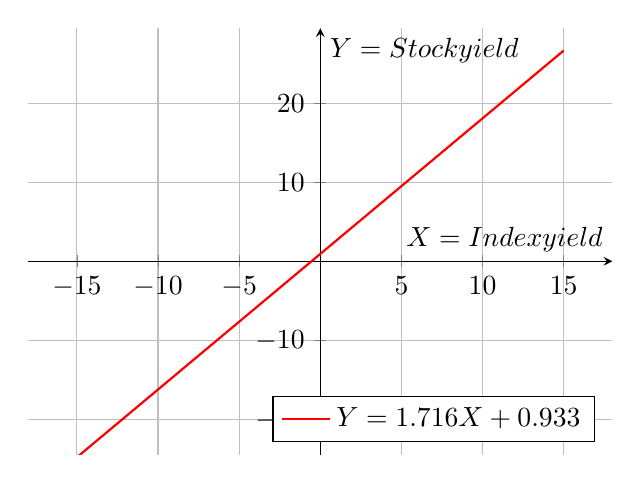
\begin{tikzpicture}
\begin{axis}[
    xlabel={$X = \text{Index yield}$},
    ylabel={$Y = \text{Stock yield}$},
    grid=both,
    axis lines=middle,
    xmin=-15, xmax=15,
    ymin=-20, ymax=25,
    width=9cm, height=7cm, % Taille réduite ici
    enlargelimits=true,
    samples=100,
    domain=-15:15,
    legend pos=south east
]

% Droite de régression
\addplot[thick, red] {1.716*x + 0.933};
\addlegendentry{$Y = 1.716X + 0.933$}

\end{axis}
\end{tikzpicture}
\caption{Regression between stock and index return}
\end{figure}
